\documentclass[12pt,a4paper]{article}
\usepackage[utf8]{inputenc}
\usepackage[T1]{fontenc}
\usepackage{geometry}
\usepackage{hyperref}
\usepackage{enumitem}
\usepackage{parskip}
\usepackage{graphicx}
\graphicspath{{./}{report/}{images/}{../images/}}

\geometry{margin=1.5cm}

\title{Project Documentation: \\ 
	Web Technologies 2025/26 Group Project}
\author{}
\date{}

\begin{document}

\maketitle

\section{Introduction}

This project implements a web platform for exploring and analysing anime-related data. Users can browse anime, characters and authors, apply filters and sorting, and submit ratings through an intuitive web interface.

The system is built using a multi-server architecture with a central Express server acting as a lightweight middleware between the client and two data services: a Spring Boot service with a PostgreSQL database for static data, and an Express service with MongoDB for dynamic data. The front-end is developed with HTML, CSS, JavaScript and Handlebars templates.

The project follows the design principles and technologies introduced in the course, focusing on modularity, clear separation of concerns and well-documented APIs.

The project startup is fully automated through Docker containers and can be executed with a single command, \texttt{./start-dev.sh} from the \texttt{solution} directory.

\begin{figure}[h]
    \centering
    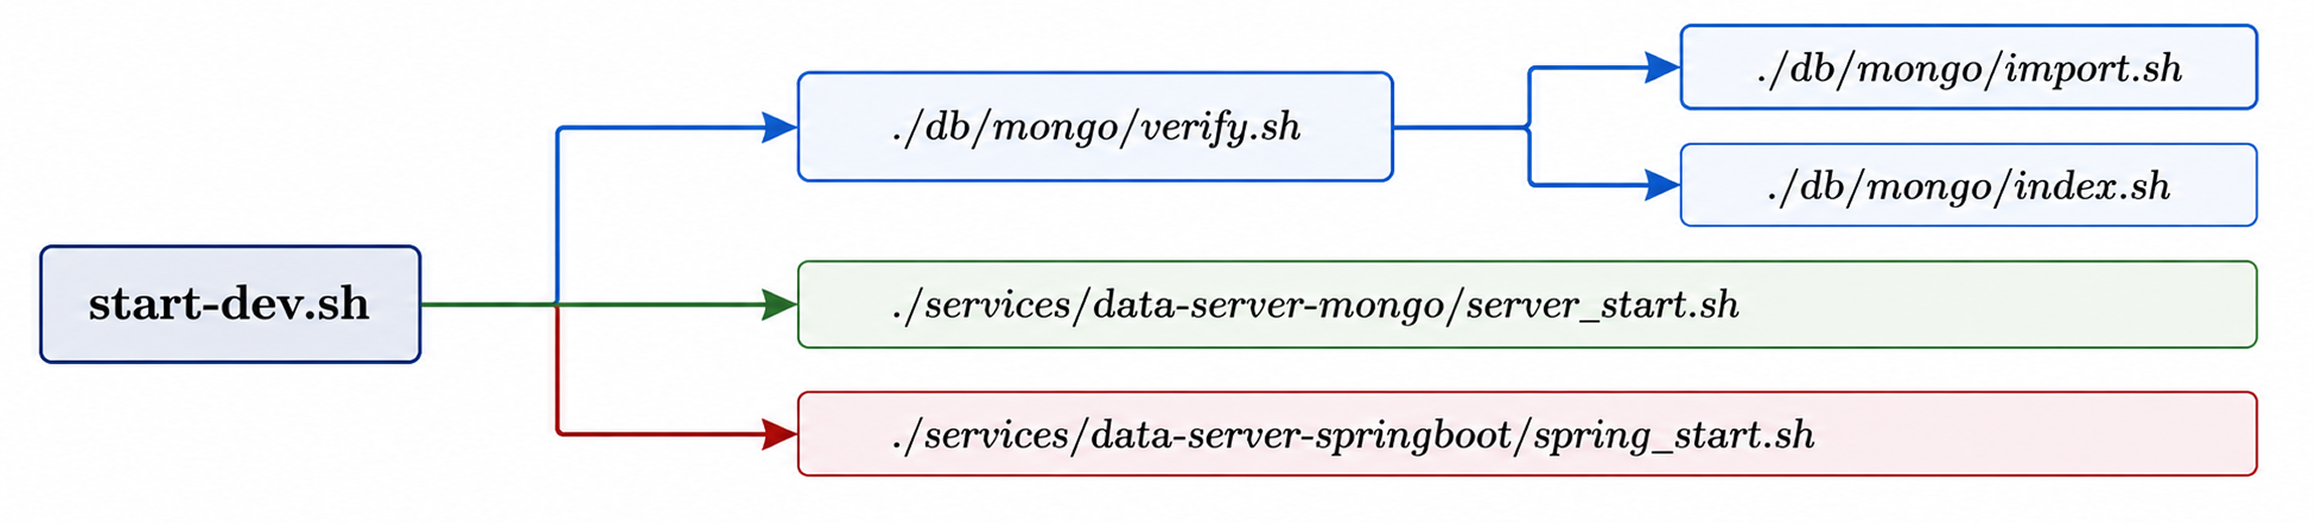
\includegraphics[width=0.9\linewidth]{images/script_scheme.png}
\end{figure}


\section{Technical Task 1 -- System Architecture and Data Management}

\subsection{Design and Motivations}

The system follows a microservice architecture with a central Express server acting as the entry point and coordinating access to two data services. Static data are stored in PostgreSQL and served by a Spring Boot application, while dynamic data are stored in MongoDB to support high write volumes. The central server communicates with both services via Axios, ensuring a clear separation of concerns and keeping the middleware lightweight. The front-end is rendered server-side using Handlebars, as required by the assignment. Docker Compose orchestrates all services, with configuration managed through environment variables and a start-up script to simplify development and data loading.

\subsection{Issues}

Major challenges included handling large datasets, indexing MongoDB collections for performance, mapping a complex relational schema in PostgreSQL, and coordinating asynchronous calls between services. Additional effort was required to validate user input and correctly configure Docker networking across environments.

\subsection{Requirements}

The architecture meets the assignment requirements by separating static and dynamic data, using Express and Spring Boot, and keeping the central server lightweight. All services expose REST APIs with pagination, filtering and sorting, are fully containerised with Docker Compose, and provide Swagger documentation.

\subsection{Limitations}

The system lacks caching, authentication and advanced error handling. Services run as single instances, limiting scalability, and cross-database queries require data composition at the central server, which may introduce latency.

\section{Technical Task 2 -- Postgres Data Service (Spring Boot)}

\subsection{Design and Motivations}

The Spring Boot service exposes REST endpoints under \texttt{/api} to deliver data from PostgreSQL. We used Spring Data JPA to map tables such as \texttt{details}, \texttt{characters}, \texttt{character\_anime\_works}, \texttt{character\_nicknames} and \texttt{person\_details} to Java entities. Controllers provide endpoints for listing resources with pagination, searching by attributes, selecting specific fields and filtering by NULL values. For example, \texttt{/api/details} returns paginated anime with filters for year, type, status, rating, genres and episodes; \texttt{/api/details/\{mal\_id\}} returns a single anime with optional field selection; and \texttt{/api/details/\{mal\_id\}/characters} returns characters appearing in an anime. Sorting accepts comma-separated fields prefixed with \texttt{-} for descending order, with NULL values always sorted last. Spring Boot's ecosystem enabled straightforward testing and comprehensive Swagger documentation.

\subsection{Issues}

Mapping the relational schema to Java entities required careful handling of composite keys (\texttt{@IdClass}) for junction tables like \texttt{CharacterAnimeWorks} and \texttt{CharacterNicknames}. We implemented custom JPQL queries with \texttt{@Query} for complex operations like JOINs and genre filtering that exceeded automatic query derivation capabilities. Converting database snake\_case to JSON snake\_case while maintaining Java camelCase required manual mapping functions in controllers. NULL value handling needed dedicated repository methods (\texttt{findByFieldIsNull}/\texttt{IsNotNull}) and special sorting logic (\texttt{.nullsLast()}) to properly manage incomplete data. Swagger annotations became verbose across 20+ endpoints but provide essential self-documentation.

\subsection{Requirements}

The Spring Boot service meets the Java server requirement with well-documented REST endpoints supporting pagination, sorting and filtering. It uses JPA for ORM, PostgreSQL for persistence, and environment variables for configuration (database host, port, credentials) passed via startup scripts. The implementation returns snake\_case field names matching the dataset structure and includes relationship endpoints for characters, voice actors and anime appearances. Swagger/OpenAPI documentation is accessible at \texttt{/swagger-ui.html} with detailed parameter descriptions and response codes for all endpoints.

\subsection{Limitations}

The service implements only basic text search (case-insensitive partial matching) without full-text indexing capabilities. Some endpoints may return large payloads when field selection is not specified. Query optimization relies on basic indexes; complex multi-table JOINs may experience latency on datasets exceeding 100,000 records. The API lacks caching, rate limiting and advanced error handling mechanisms that would be expected in production systems.

\section{Technical Task 3 -- MongoDB Data Service (Node.js)}

\subsection{Design and Motivations}

The MongoDB service is a Node.js application using Express and native MongoDB drivers. It manages the three dynamic collections: \texttt{ratings}, \texttt{favs} and \texttt{stats}. The \texttt{/api/ratings} endpoint allows clients to retrieve ratings by anime identifier, filter by score ranges and paginate results. Clients can also submit ratings via a POST request; the service writes the new rating and updates the corresponding aggregate statistic (e.g.\ average score and vote counts). All endpoints return data with optional filters. We defined a service layer to encapsulate MongoDB operations and controllers to handle HTTP requests, ensuring separation of concerns and making the code testable.

\subsection{Issues}

The primary challenges in this service were related to data volume and consistency. The ratings collection alone contains hundreds of millions of documents, so queries must use indexes to avoid full collection scans. Creating these indexes during deployment adds several minutes to the setup process. When users submit new ratings, we need to validate the request and check that the username exists in the PostgreSQL database; the service delegates this check to the central server's API client, introducing latency. Updating aggregate statistics in MongoDB requires careful handling to avoid race conditions; we chose to fetch the current statistic document, compute the new values and write them back atomically. Ensuring that our API adheres to REST principles while also providing flexibility for advanced queries required designing a consistent parameter scheme (e.g.\ \texttt{minScore} and \texttt{maxScore} for numeric filters).

\subsection{Requirements}

This service fulfils the requirement to store dynamic data in MongoDB and to implement at least one server in Node.js. It exposes REST endpoints for retrieving and creating ratings, favourites and statistics, uses pagination and supports advanced filtering options. The service is documented with swagger-jsdoc and served at \texttt{/api-docs}. Environment variables specify the MongoDB connection string and server port. Data import scripts populate the collections and create indexes; the README explains how to run these scripts. The service integrates with the central server by accepting \texttt{username}, \texttt{anime\_id} and \texttt{score} fields for new ratings and returns the updated average score to the client. Proper status codes and error messages are returned for missing data or invalid requests.

\subsection{Limitations}

Current queries on the ratings collection rely on simple comparison operators and do not support more complex aggregations such as time-series analysis or grouping by user. Our POST endpoint for ratings does not yet support updating existing ratings; repeated submissions create duplicate documents. The service trusts the central server's validation and does not implement its own user authentication. While our design includes indexes on frequently queried fields, the large size of the collections still results in non-trivial response times, especially on commodity hardware. Additional caching, concurrency controls and transaction support would be necessary for production use.

\section{Technical Task 4 -- Central Express Server and Front-end}

\subsection{Central Server -- Design and Motivations}

The central server is implemented in Node.js using Express and Handlebars and acts as the main entry point for user interaction. It serves as a lightweight middleware between the client and two back-end data services (Spring Boot/PostgreSQL and Express/MongoDB), complying with the assignment requirement to avoid heavy computation. Communication with the data services is handled via Axios clients, and routes such as \texttt{/anime}, \texttt{/anime/:id}, \texttt{/anime/:id/ratings} and \texttt{/profile/:username} translate user requests into appropriate API calls. Handlebars templates with partials and helpers are used for server-side rendering of lists, filters and pagination while preserving query parameters across navigation. This approach simplifies the front-end stack and ensures full compliance with the assignment constraints. Compared to a React-based solution, server-side rendering with Handlebars reduces client-side complexity and avoids the need for a separate front-end build process, but it limits interactivity and prevents dynamic UI updates without page reloads.

\subsection{Issues}

Key challenges included mapping user input into valid API queries while preserving active filters across pagination. Input validation and normalisation were required before forwarding requests to the data services. Some pages require data aggregation from both PostgreSQL and MongoDB, which involved coordinating multiple asynchronous calls and handling partial service failures. Fallback mechanisms were implemented to ensure static content remains available when dynamic data cannot be retrieved. Designing a clear interface using only HTML and Handlebars required careful layout planning. The absence of caching at this level means that performance depends on network latency and back-end response times.

\subsection{Requirements}

The central server satisfies the assignment requirements by using Express as the main gateway and Handlebars for templating. It supports filtering, sorting and pagination aligned with the underlying APIs. Configuration is managed via environment variables, including service URLs and logging options. Rating submission is handled through POST forms, with username validation delegated to the PostgreSQL service before forwarding data to MongoDB. Static assets are served directly, and all routes are documented using Swagger to ensure clarity and maintainability, while the code has been documented with jsDoc.

\subsection{Limitations}

The application does not implement authentication or advanced personalisation features. UI interactions are page-based and lack dynamic behaviours such as live filtering or auto-complete, which a React front-end could provide. Requests are forwarded sequentially without caching or batching, limiting scalability under heavy load. While the chosen architecture ensures simplicity and robustness, a React-based client could offer a more responsive user experience at the cost of increased architectural and implementation complexity.

\section{Conclusions}

Building a multi-service web application that integrates relational and document-oriented data taught us valuable lessons about system design, data modelling and cross-technology integration. We realised early on that clear separation of concerns and consistent API design make it easier to manage complexity. Containerisation with Docker simplified deployment and allowed us to replicate the environment across different development machines. Handling large datasets required tuning indexes and writing efficient queries; we learned to measure performance. Collaboration across different programming languages fostered better teamwork, as each member had to understand how their component interacted with the others. While our implementation meets the essential requirements, numerous opportunities remain for improvement, such as adding authentication with password managment and caching.

\section{Division of Work}

We divided tasks to leverage each member's strengths while ensuring that everyone contributed to all parts of the project.\\
Member Alasotto Cristian focused on the central Express server and front-end, designing the Handlebars templates, implementing route logic, ensuring that query parameters were correctly mapped to API calls, and creating and managing the Docker containers used to run the project services.\\
Member Collura Federico took primary responsibility for the Spring Boot service, modelling the PostgreSQL schema in Java, writing custom queries and integrating Swagger documentation.\\
Member Correndo Davide led the development of the MongoDB service, writing controllers and services for ratings, favourites and statistics, and implementing data import and indexing scripts.\\

\section{Extra Information}

To run the system, ensure that Docker and Node.js are installed and that the dataset files are placed in the \texttt{solution/data} folder. For the simplest setup, navigate to the \texttt{solution} directory and run \texttt{./start-dev.sh}; this script starts the databases, imports the PostgreSQL data and launches all services. Alternatively, you can start the containers manually using \texttt{docker compose up}, install dependencies in the \texttt{main-server-express} directory and run \texttt{npm run dev}. MongoDB collections can be populated using \texttt{./db/mongo/import.sh} and indexed with \texttt{./db/mongo/index.sh}; the script \texttt{./db/mongo/verify.sh} checks that the counts of documents match the expected totals. The system uses environment variables defined in \texttt{.env} to configure service URLs and logging levels. Once running, the web interface is accessible at \url{http://localhost:3000}.

\end{document}
